\ttpfig{fig:fit}{Model Fit Measures}{
    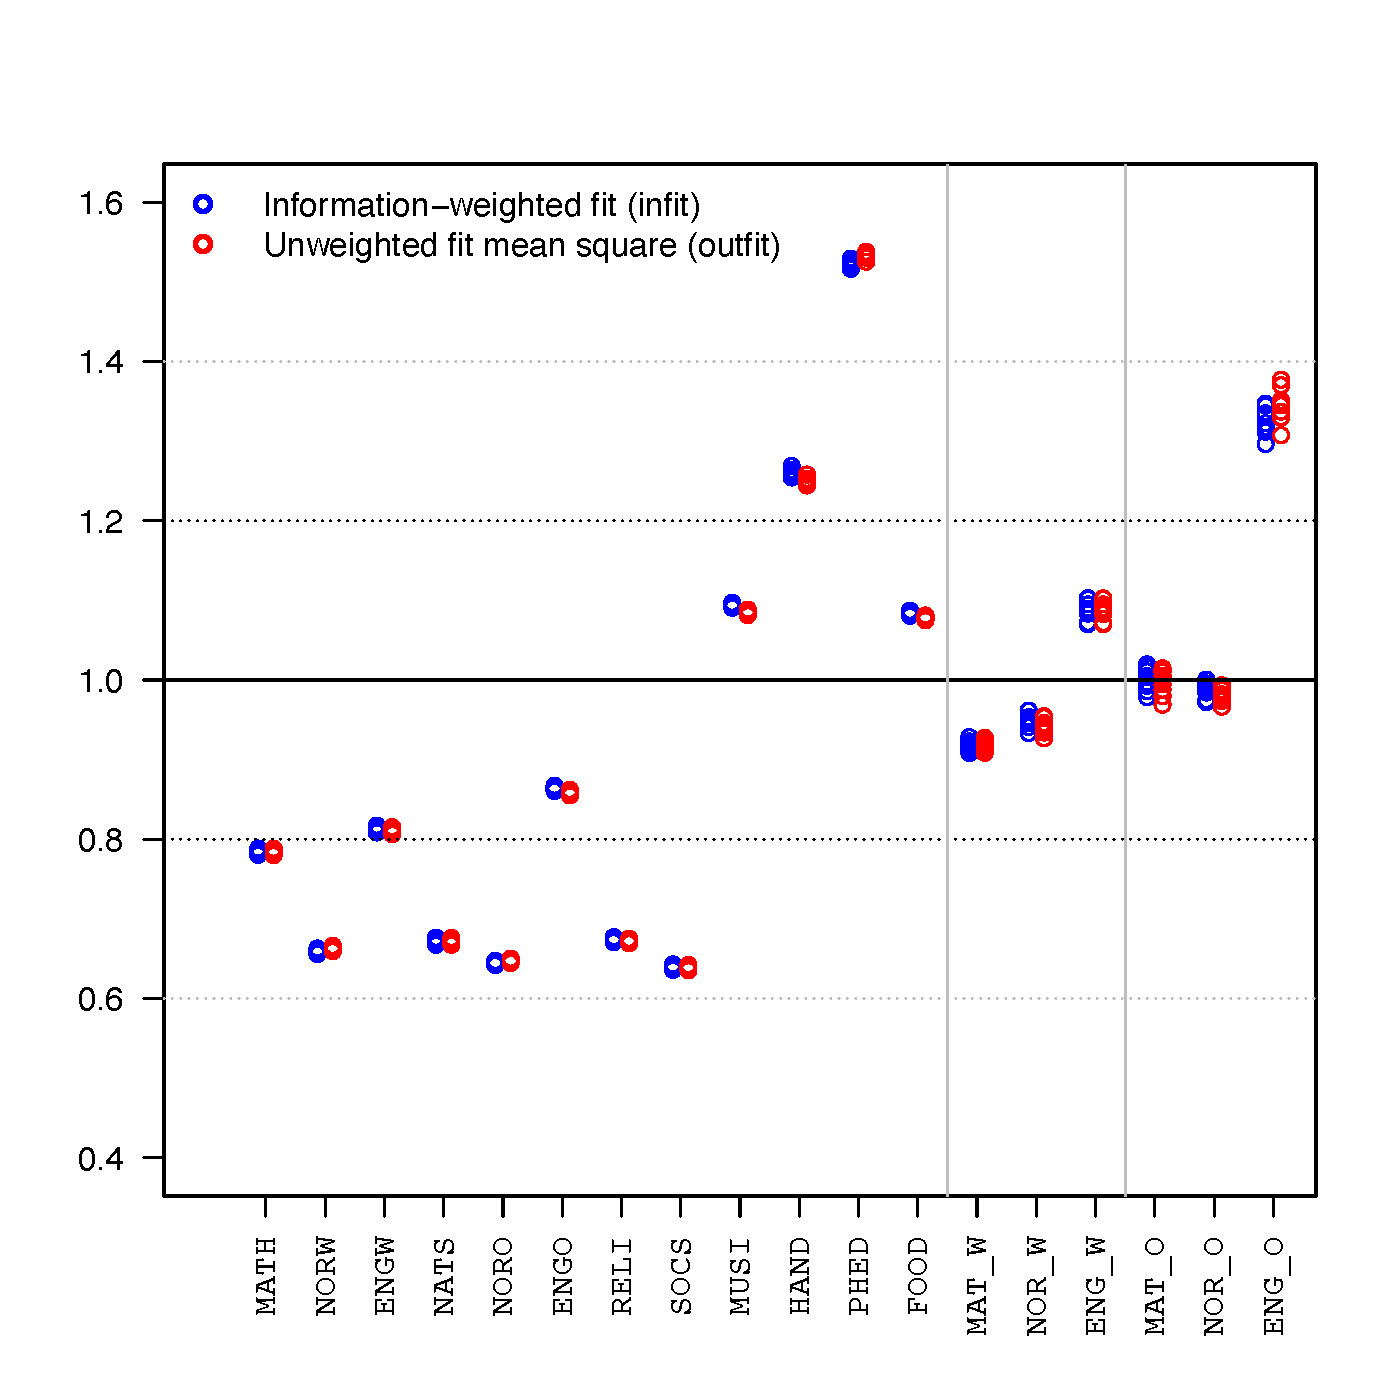
\includegraphics[width=\textwidth]{./Figures/fit.png}
}{A perfectly fit item in a Rasch model corresponds to infit and outfit statistics of $1$. Fit measure below $1$ indicate overfit where the item is more discriminating than the average item discrimination. Overfitting is usually not a problem comparing with underfitting. Empirical rules suggests close examination of items with infit and outfit statistics between $1.2$ and $1.5$ \parencite{wu:2016}. By this criterion, \textsc{hand} and \textsc{phed} fit poorly into ``\emph{the} general scholastic aptitude'' construction of \textsc{gpa}. Oral English exam is also deviating from the \textsc{gpa} model.}
